\section{Methods}

\textbf{Problem Formulation.} As input, RNAFlow receives the protein backbone atom structure $\vec P \in \mathbb{R}^{L_p\times3\times3}$, where $L_p$ is the number of residues, and each residue contains backbone atoms $N$, $C_\alpha$, and $C$. The protein sequence is also given as input where a single token is $p_i$, $i \in \{0, 1, 2, \ldots, L_p - 1\}$. The model is trained to predict RNA sequence with tokens $r_i$, $i \in \{0, 1, 2, \ldots, L_r - 1\}$. The model also predicts RNA backbone structure $R \in \mathbb{R}^{L_r\times3\times3}$, where $L_r$ is the number of nucleotides, and each nucleotide contains backbone atoms $P$, $C_{4}'$, and $N_{1}/N_{9}$ (pyrimidine/purine)~\citep{wadley2007evaluating}.

\textbf{Background: Conditional Flow Matching.} By the flow matching framework~\cite{lipman2022flow}, consider data distribution $p_1$ of RNA backbone structures and a prior distribution $p_0(\vec R | \vec R_1)$, where $\vec R_1$ is a sample from $p_1$. A \textit{flow} transforms $p_0$ to $p_1$, and this flow can be parameterized by a sequence of time-dependent conditional probability paths $p_t(\vec R_t | \vec R_1)$, $t \in [0,1]$. A sample from $p_t$ can be computed by linear interpolation, as given by Equation \hyperref[interpolation]{1}, where $\vec R_0$ is a sample from the prior distribution.

\begin{equation}\label{interpolation}
\vec R_t | \vec R_1 = (1 - t) * \vec R_0 + t * \vec R_1
\end{equation}

This probability path is generated by a marginal vector field that defines how individual samples are transported. We can define this vector field as given in Equation \hyperref[vecfield]{2}, and we can integrate over the field from time $0$ to time $1$ to generate samples from $p_1$ given a noise sample from $p_0$.

\begin{equation}\label{vecfield}
\hat v (\vec R_t; \theta) = \frac{\hat R_1(\vec R_t; \theta) - \vec R_t}{1 - t}
\end{equation}

We aim to learn this vector field by approximating $\hat R_1$ with a neural network trained with the reparameterized conditional flow matching objective. Particularly, as with diffusion, the neural network can conveniently be trained to predict samples from the data distribution given noised sample $\vec R_t$.

We choose to employ flow matching rather than the related diffusion framework \cite{ho2020denoising}, primarily due to computational efficiency. Diffusion inference often requires thousands of forward passes to generate quality samples. Since our score model involves a large structure prediction network, RNAFlow inference time would be much slower in a diffusion setting \cite{yim2023fast}. In contrast, quality samples can be generated by flow matching with a much fewer number of passes. 

\subsection{RNAFlow Algorithm: Overview}

We generate RNA sequences and structures using a conditional flow matching model where the score predictor is an inverse folding denoiser and pre-trained folding network. The inverse folding denoiser, which we refer to as \textbf{Noise-to-Seq}, is a geometric graph neural network conditioned on protein structure and sequence. Noise-to-Seq is pre-trained on the RNA inverse folding task and subsequently fine-tuned on the flow matching objective. It follows the RNA inverse folding architecture presented by \citet{joshi2023multi}, which is detailed in section \hyperref[sec:3.2]{3.2}.

\textbf{Initialization}. As our prior distribution, we choose a unit Gaussian on $\mathbb{R}^3$ centered at zero, from which we sample $\vec R_0$. We also translate the true protein-RNA complex [$\vec P_1$, $\vec R_1$] such that the center of mass of $\vec R_1$ is zero. As shown in Algorithm \hyperref[rnaflow:train]{1}, we Kabsch align \cite{kabsch1976solution} the sampled noise $\vec R_0$ with the true RNA $\vec R_1$ to eliminate global rotations, leading to faster training convergence \cite{klein2023equivariant}. By this approach, we train with the ground-truth pose of the protein relative to the RNA centroid, though this is not leaked at inference time.

\begin{algorithm}[t]
\caption{RNAFlow: Train}\label{rnaflow:train}

\algorithmicrequire $\{p_i\}_{\forall i}$, $\{r_i\}_{\forall i}$, $[\vec P_1, \vec R_1]$
\vspace{0.25em}

Sample prior $\vec R_0 \sim \mathcal{N}(0, I_3)^{L_r}$
\vspace{0.25em}

Kabsch align noise $\vec R_0$ with true backbone $\vec R_1$
\vspace{0.25em}

Sample timestep $t \sim \text{Uniform}[0, 1]$
\vspace{0.25em}

Interpolate $\vec R_t \gets t * \vec R_1 + (1 - t) * \vec R_0$
\vspace{0.25em}

Predict $\{\hat r_i\}_{\forall i} \gets \text{\textbf{Noise-to-Seq}} \{ [\vec P_1, \vec R_t], \{p_i\}_{\forall i}, t \}$ 
\vspace{0.25em}

Predict $\hat R_1 \gets \text{RF2NA} \{ \{\hat r_i\}_{\forall i} \} $

\end{algorithm}

\textbf{Training}. During training, we sample a timestep $t$ and interpolate the true RNA backbone with the sampled prior to arrive at noised backbone $\vec R_t$. The true protein backbone, noised RNA backbone, and protein sequence are given as input to Noise-to-Seq which predicts a denoised RNA sequence. RF2NA folds the predicted RNA sequence into predicted structure $\hat R_1$. This process is shown in Figure \ref{fig:1}.

The outputs of an RNAFlow training pass are an RNA sequence and its structure. The reparameterized flow matching objective gives that the score model should be trained with a standard $L_2$ loss. Therefore, as given in Equation \hyperref[loss]{3}, we compute the MSE between all predicted and true RNA backbone coordinates. Before MSE computation, we Kabsch align the two RNA backbones, since we are optimizing for RNA structure design rather than docking accuracy. Additionally, we supervise the sequence with a cross entropy loss between predicted and true nucleotide types.

\begin{equation}\label{loss}
\mathcal{L} = \text{MSE}(\hat R_1, \vec R_1) + \sum_i \text{CE}(\hat r_i, r_i)
\end{equation}

The sequence output from Noise-to-Seq is used as input to RF2NA, and the resulting structure is supervised to update the weights of the model. Since gradients must propagate between Noise-to-Seq and RF2NA, we apply the Gumbel-Softmax estimator to differentiably sample from the predicted logits \cite{jang2016categorical}. Further justification of this objective is given in the Appendix. 

\textbf{Inference: RNAFlow-Base}. As shown in Algorithm \hyperref[rnaflow:inference]{2}, we begin by generating a ``pose guess'' using RF2NA. Specifically, we fold the protein MSA with a mock RNA sequence consisting of all adenines, of the same length as the true RNA sequence. The predicted complex is used as an initial guess of protein pose with respect to the RNA centroid. $\vec P_0$ is the true protein backbone Kabsch-aligned onto the predicted protein pose, and $\vec R_0$ is drawn from the prior distribution. RNAFlow refines its predictions over multiple steps, predicting the true complex [$\hat P_1$, $\hat R_1$] on each iteration. The final outputs of RNAFlow inference are a predicted RNA sequence and structure.

\textbf{Inference: RNAFlow-Traj}. In standard RNAFlow inference, Noise-to-Seq predicts a sequence based on a single RNA structure. However, an RNA backbone structure can adopt multiple conformations, and it is important that the final RNA sequence reflects this conformational diversity \cite{ganser2019roles}. Indeed, \citet{joshi2023multi} demonstrates that inverse folding on a set of RNA conformations improves the native sequence recovery rate compared to single-structure model.
To this end, we propose to generate a final RNA sequence by conditioning on multiple RNA structures generated over the course of flow matching inference. This inverse folding model, referred to as \textbf{Trajectory-to-Seq (Traj-to-Seq)}, is a multi-graph neural network which can handle multiple RNA conformation inputs. Its architecture is detailed in section \hyperref[sec:3.3]{3.3}.

% placement
\begin{algorithm}[h]
\caption{RNAFlow-Traj: Inference}\label{rnaflow:inference}

\algorithmicrequire $\{p_i\}_{\forall i}$, $\vec P_1$
\vspace{0.25em}

Position $\vec P_0$ by aligning $\vec P_1$ with RF2NA pose guess
\vspace{0.25em}

Sample prior  $\vec R_0 \sim \mathcal{N}(0, I_3)^{L_r}$
\vspace{0.25em}

Initialize $traj \gets []$
\vspace{0.25em}

\algorithmicfor {$n \gets 1$ \textbf{to} $N$}
\vspace{0.25em}

    \hspace{0.2in} Let $t_2 \gets n/N$ and $t_1 \gets (n-1)/N$
    \vspace{0.25em}
    
    \hspace{0.2in} $\{\hat r_i\}_{\forall i} \gets \text{\textbf{Noise-to-Seq}} \{ [\vec P_{t_1}, \vec R_{t_1}], \{p_i\}_{\forall i}, t_1 \}$
    \vspace{0.25em}
    
    \hspace{0.2in} Predict [$\hat P_1$, $\hat R_1] \gets \text{RF2NA} \{ \{\hat r_i\}_{\forall i}, \text{protein MSA} \}$
    \vspace{0.25em}
    
    \hspace{0.2in} Append $\hat R_1$ to $traj$
    \vspace{0.25em}
    
    \hspace{0.2in} Interpolate $\vec R_{t_2} \gets \vec R_{t_1} +  \frac{(\hat R_{1} - \vec R_{t_1})}{(1 - t_1)} * (t_2 - t_1)$
    
    \hspace{0.2in} Align $\vec P_{t_2} \gets \text{Kabsch}(\vec P_1, \hat P_1)$
    
\algorithmicendfor

Predict $\{\hat r_i\}_{\forall i} \gets \text{\textbf{Traj-to-Seq}} \{ traj \}$
\vspace{0.25em}

\textbf{Outputs:} $\{\hat r_i\}_{\forall i}$, $traj[-1]$

\end{algorithm}

\subsection{Noise-to-Seq Module}
\label{sec:3.2}

Noise-to-Seq is a graph-based RNA inverse folding model, fine-tuned to predict RNA sequences autoregressively from noised structures. As in \citet{ingraham2019generative} and \citet{jing2021equivariant}, the model applies an encoder-decoder architecture where the encoder learns a representation of the protein-RNA complex structure and the decoder predicts a distribution over nucleotides at each position $i$, given sequence information of all positions before $i$.

\textbf{Graph Representation.} We represent each backbone 3D point cloud [$\vec P$, $\vec R$] as a graph $\mathcal{G} = (\mathcal{V}, \mathcal{E})$. Each amino acid $i$ is assigned a node at $C_\alpha$ coordinate $\vec{x_i} \in \vec P$, and each nucleotide $j$ is assigned a node at $C_{4}'$ coordinate $\vec{x_j} \in \vec R$. Node features are denoted as $\mathcal{V} = \{ v_1, \ldots, v_{L_p + L_r} \}$. As shown in Figure \hyperref[fig:1]{1}, for all nodes $\vec{x}_i \in \vec P$, we draw edges to $10$ nearest neighbor nodes whose 3D coordinates are also in $\vec P$. Likewise for all nodes $\vec{x}_i \in \vec R$, we draw edges to $10$ nearest neighbor nodes whose 3D coordinates are also in $\vec R$. For all nodes $\vec{x}_i \in \vec P$, we additionally draw edges to $5$ nearest neighbor nodes $\vec{x}_j \in \vec R$. Nearest neighbors are computed by $\Vert \vec{x}_i - \vec{x}_j \Vert_2$. Edge features are denoted as $\mathcal{E} = \{ e_{i,j} \}_{i \neq j}$.

\textbf{Node \& Edge Features}. We compute node features and edge features as follows. Node vector features include unit vectors to neighboring nodes on the backbone chain and unit vectors to the remaining two atoms of the nucleotide ($P$ and $N_{1}/N_{9}$) or amino acid ($N$ and $C$). Node scalar features include magnitudes of all vector features, encoded by radial basis functions, and a one hot encoding of residue identity for the protein chain. Edge vector features include a unit vector from the source node to the destination node, and its magnitude encoded by radial basis functions is a scalar feature. Edge scalar features also include distance along the backbone between the source and destination, encoded with a sinusoidal embedding. If the edge connects nodes in two different chains, the encoded number is equal to $L_p+L_r$.

% placement
\begin{figure*}[ht]
    \centering
    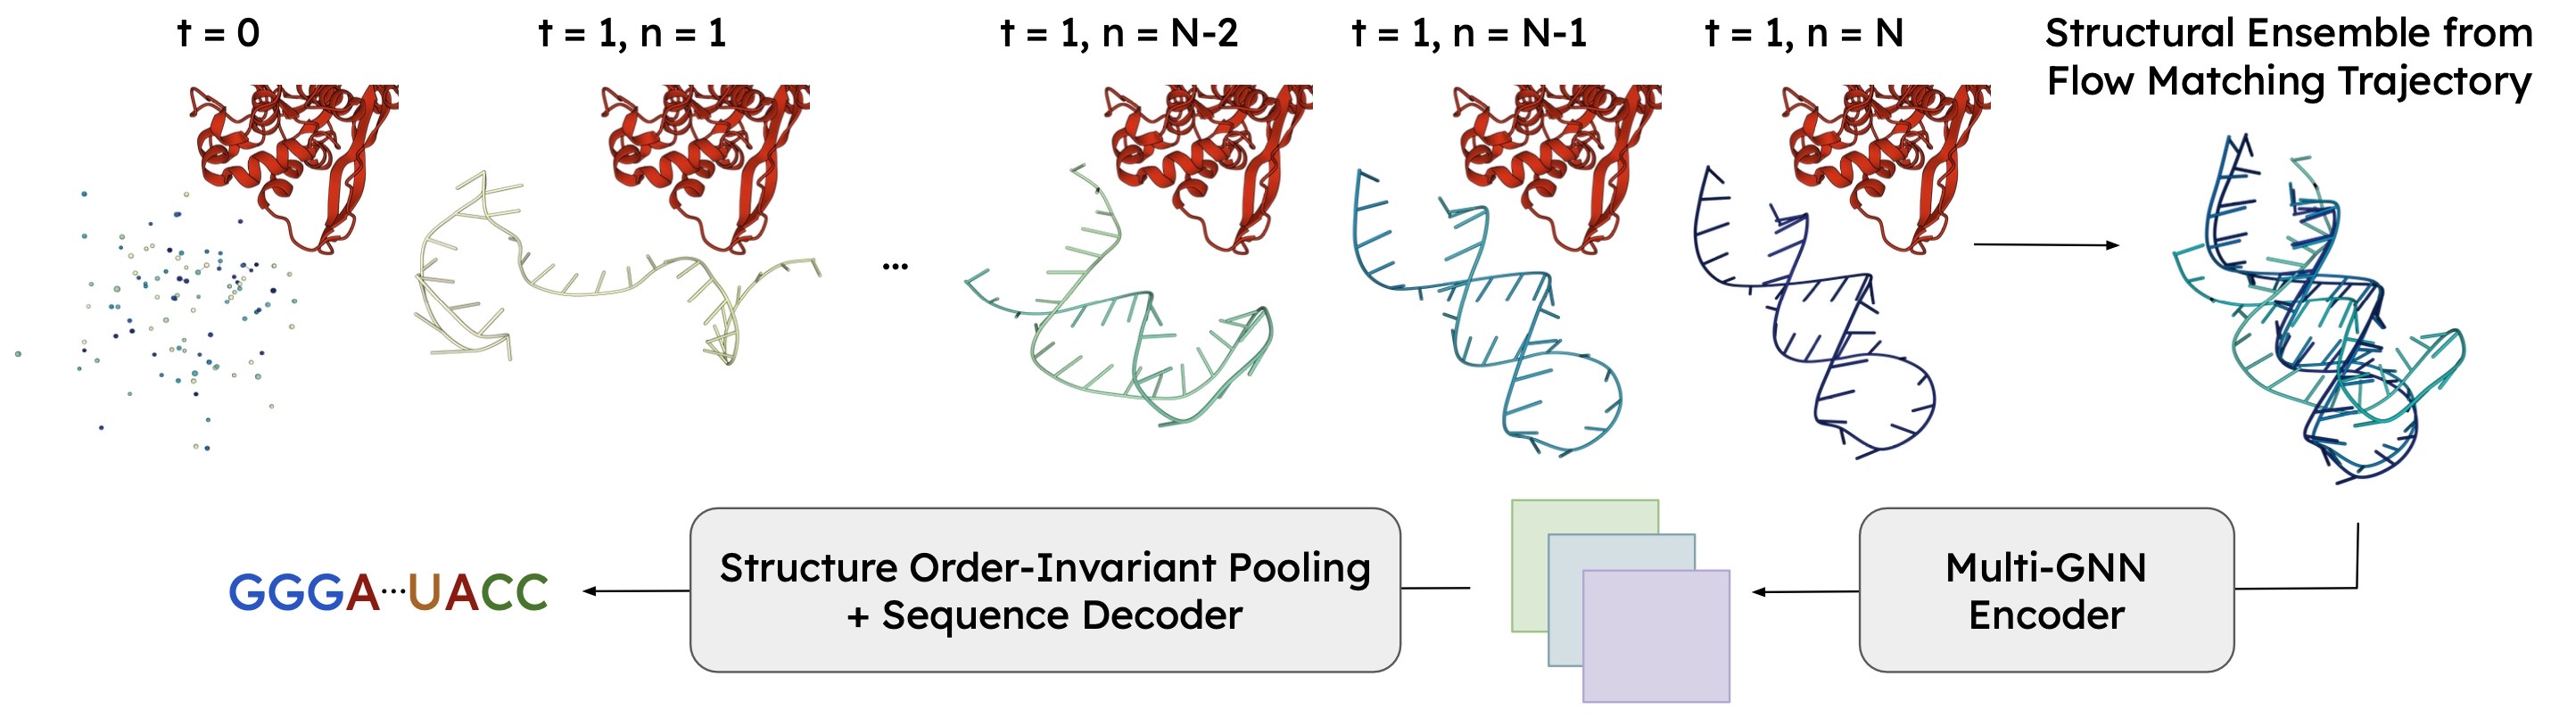
\includegraphics[width=2\columnwidth]{traj-to-seq.png}
    \caption{One forward pass during Traj-to-Seq inference. A subset of structures from a flow matching trajectory are encoded by a multi-GNN and pooled in an order-invariant manner to predict an RNA sequence.}
    \label{fig:2}
\end{figure*}

\textbf{Model Architecture.} Noise-to-Seq contains a message-passing encoder consisting of GVP-GNN layers \cite{jing2020learning}. First, input node features $v_i$ and edge features $\{ e_{i,j} \}_{i \neq j}$ are encoded by GVPs.
\begin{align*}
h_{v_i} &= g_v ( \text{LayerNorm} (v_i) )  \\
h_{e_{i,j}} &= g_e ( \text{LayerNorm} (e_{i,j}) ) 
\end{align*}
Node embedding GVP $g_v$ and edge embedding GVP $g_e$ apply the vector gating strategy proposed by \citet{jing2021equivariant}. If the input structure is noised, we add a timestep embedding to the node features, encoded by random Fourier features of size $256$ \cite{tancik2020fourier} and concatenated onto the scalar component of $h_{v_i}$. For every position $i$, $h_{v_i}$ is residually updated by a sequence of three message-passing layers where each layer has the following architecture:
\begin{align*}
m_{v_i} &= \frac{1}{|\mathcal{N}|} \sum_{j \in \mathcal{N}} g_{MSG} (h_{v_i}, h_{v_j}, h_{e_{i,j}})  \\
h_{v_i}^{'} &= \text{LayerNorm} (h_{v_i} + \text{Dropout}(m_{v_i})) \label{update}
\end{align*}
$g_{MSG}$ is a sequence of three GVPs with vector gating and ReLU activation on the scalar features. After each message-passing layer, we also apply pointwise feedforward updates to the node embedding.
\begin{align*}
h_{v_i}^{'} = \text{LayerNorm} (h_{v_i}^{'} + \text{Dropout}(g_{FF}(h_{v_i}^{'})))
\end{align*}
$g_{FF}$ is a sequence of two GVPs with vector gating and the ReLU activation on the scalar features. We then encode protein and RNA sequence information with an embedding layer and concatenate these features onto the edge scalar features. By the autoregressive scheme, we mask out sequence features for edges where the source node's position is greater than the destination node's position. The protein nodes are always positioned before RNA nodes, so protein sequence context is always present during decoding. Our decoder's architecture is identical to the encoder, except that messages are aggregated by a sum instead of a mean. Finally, we apply a GVP layer and softmax to predict probabilities of the $4$ nucleotide classes at each position. The model is supervised by a cross entropy loss between the true RNA sequence and predicted nucleotide probabilities.

\subsection{Traj-to-Seq Module}
\label{sec:3.3}

As shown in Figure \hyperref[fig:2]{2}, the flow matching inference loop generates a trajectory of RNA structures over iterative refinement steps. Traj-to-Seq is a graph-based inverse folding model that predicts RNA sequences based on the output trajectory of a single RNAFlow inference pass. At the final stages of the trajectory, the structures have a high degree of secondary structure similarity while displaying variation in tertiary structure, qualitatively resembling a conformational ensemble \cite{fornili2013specialized}. Therefore, we can leverage the outputs of a single flow matching inference pass as a conformational ensemble approximation.

\textbf{Model Inputs.} We represent a trajectory of RNA backbones as a set of independent graphs  \{$\mathcal{G}^{(1)}, ..., \mathcal{G}^{(k)}$\} where $k$ is the number of conformers. Traj-to-Seq does not accept protein information as input, so each node in $\mathcal{G}^{(n)}$ corresponds to a nucleotide $j$ at $C_{4}'$ coordinate $\vec{x_j} \in \vec R^{(n)}$. For all nodes $\vec{x}_j \in \vec R^{(n)}$, we draw edges to $10$ nearest neighbor nodes whose 3D coordinates are also in $\vec R^{(n)}$, so edges are not drawn between conformers. Instead, Traj-to-Seq is designed to operate on ``multi-graphs.'' As introduced by \citet{joshi2023multi}, a multi-graph is constructed by stacking each RNA graph's scalar and vector features and building a joint adjacency matrix, computed as the union of each individual graph's adjacency matrix.

\textbf{Architecture.} Traj-to-Seq employs the same encoder-decoder architecture as Noise-to-Seq. The GVP encoder processes each structure independently, such that $h_{v_i} \in \mathbb{R}^{k \times f}$ where $k$ is the number of conformers and $f$ is the feature dimension. A merged representation is computed by a structure order-invariant mean. Finally, a decoder identical to Noise-to-Seq is employed to predict RNA sequence. 

\subsection{Output Rescoring Model}

Since RNAFlow can be sampled many times to obtain several RNA designs, we train an \textit{output rescoring model} to select from amongst the samples based on predicted recovery rate. For training, we generate 6 mutated RNA sequences for each ground-truth protein-RNA complex. Binary labels are generated based on whether or not a generated RNA sequence has a recovery rate $\geq 30\%$. At test time, we evaluate many RNAFlow output samples for a single protein and make selections based on the highest predicted probability of a positive outcome, prioritizing designs with the greatest likelihood of achieving a recovery rate of at least $30\%$.

The inputs to the output scoring model are protein sequence, protein structure, RNA sequence, and RF2NA-folded RNA structure. The protein and RNA are each encoded by a GVP model with the same architecture as the Noise-to-Seq encoder, and the resulting node-level representations are averaged and processed by a feed-forward network. The output is supervised by a binary cross entropy loss. Hyperparameter and training details are included in the Appendix.